\documentclass[10pt,openany,a4paper]{article}
\usepackage{graphicx} 
\usepackage{multirow}
\usepackage{enumitem}
\usepackage{amssymb}
\usepackage{amsmath}
\usepackage{amsthm}
\usepackage{xcolor}
\usepackage{multicol}
\usepackage{multirow}
\usepackage{array}
\usepackage{animate}
\usepackage{amsthm}
\usepackage{caption}
\usepackage{minted}
\usepackage{fancyhdr}
\usepackage{listings}
\usepackage{tikz}
\usepackage{geometry}
	\geometry{
		total = {160mm, 237mm},
		left = 30mm,
		right = 35mm,
		top = 35mm,
        bottom = 30mm,
        headheight=2cm
	}
\usepackage{hyperref}
\hypersetup{
    colorlinks=true,
    linkcolor=blue,
    filecolor=magenta,      
    urlcolor=cyan,
    pdftitle={Overleaf Example},
    pdfpagemode=FullScreen,
    }
\renewcommand{\headrulewidth}{0pt}

\graphicspath{{C:/Users/teoso/OneDrive/Documents/Tugas Kuliah/Template Math Depart/}}

\newcommand{\R}{\mathbb{R}}
\newcommand{\N}{\mathbb{N}}
\newcommand{\Z}{\mathbb{Z}}
\newcommand{\Q}{\mathbb{Q}}
\newcommand{\jawab}{\textbf{Solusi}:}

\newtheorem*{teorema}{Teorema}
\newtheorem*{definisi}{Definisi}

\definecolor{HIMAmuda}{HTML}{01D1FD}
\definecolor{HIMAtua}{HTML}{02016A}
\definecolor{HIMAabu}{HTML}{CBCBCC}
\definecolor{pgray}{rgb}{0.5,0.5,0.5}
\definecolor{pblue}{rgb}{0.13,0.13,1}
\definecolor{pgreen}{rgb}{0,0.5,0}
\definecolor{pred}{rgb}{0.9,0,0}
\definecolor{pgrey}{rgb}{0.46,0.45,0.48}
\definecolor{pcyan}{HTML}{D4EFFC}
\definecolor{lblue}{HTML}{00AEEF}
\definecolor{input}{HTML}{AAE1FA}
\definecolor{bg}{rgb}{0.95, 0.95, 0.92}
\definecolor{vscode}{HTML}{282A36}
\definecolor{PastelGreen}{HTML}{77DD77}

\lstdefinestyle{output}{
    language=Java,
    backgroundcolor     =\color{vscode},
    basicstyle          =\footnotesize\ttfamily\color{white},
    frame               =shadowbox,
    escapeinside        ={(*}{*)},
    showspaces          =false,
    showtabs            =false,
    breaklines          =true,
    showstringspaces    =false,
    breakatwhitespace   =true,
    rulesepcolor        =\color{HIMAtua!50!white},
    rulecolor           =\color{HIMAtua!50!white},
    numbers             =none,
    }

\newcommand{\enter}{\raisebox{-1.8pt}{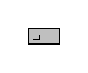
\begin{tikzpicture}[scale=0.2]
    \draw[thin,fill=lightgray] (0,0) rectangle (2,1);
    \draw (0.3,0.3) -- (0.7,0.3)--(0.7,0.6);     
\end{tikzpicture}}}

\newcommand{\inputscan}[1]{\raisebox{0pt}[1pt]{\colorbox{darkgray}{#1}}}

\pagestyle{fancy}
\fancyhf{}
\fancyhead[L]{\includegraphics[width=1.6cm]{Provicom.png}}
\fancyhead[C]{\textbf{\MakeUppercase{Pembahasan Latihan EAS}\\ 
                \MakeUppercase{Alpro 1 Kelompok 1}\\ 
                \MakeUppercase{Lab. pemrograman dan komputasi visual}\\ 
                \MakeUppercase{Departemen Matematika - FSAD ITS}}}
\fancyhead[R]{\includegraphics[width=1.6cm]{provicomIG.png}}
\begin{document}
\begin{enumerate}
    \item Perhatikan bahwa bentuk rekursif dari program adalah menghapus indeks ke-\texttt{0} dan ke-\texttt{n-1} dari string sehingga panjang string akan menjadi lebih kecil sebanyak 2 untuk setiap iterasi rekursif. Karena string minimal mempunyai panjang 0 atau string kosong, dari hal itu kita bisa membuat sebuah kesimpulan kecil berikut:
    \begin{itemize}
        \item Jika panjang string genap, maka string akhir yang akan dicek adalah string kosong.
        \item Jika panjang string ganjil, maka string akhir yang akan dicek adalah string dengan panjang 1.
    \end{itemize}
    Berarti kita bisa membuat program akan mengeluarkan \texttt{true} jika panjang string adalah 0 atau 1. Namun hal tersebut harus diasumsikan bahwa string yang diinputkan adalah palindrome. Jika tidak, maka program akan mengeluarkan \texttt{false} jika karakter pertama dan terakhir string di salah satu iterasi rekursif tidak sama. Berikut adalah implementasi dari algoritma tersebut:
    \begin{minted}[frame=lines,
        framesep=2mm,
        baselinestretch=1.2,
        bgcolor=bg,
        fontsize=\footnotesize,
        linenos]{java}
public static boolean isPalindrome(String s) {
    if (s.length() <= 1) return true;
    if (s.charAt(0) != s.charAt(s.length() - 1)) return false;
    return isPalindrome(s.substring(1, s.length() - 1));
}
    \end{minted}
    \item Soal yang cukup mudah. Untuk $n>0$ maka kita hanya tampilkan angka $n$ beserta tambahan string koma dan panggil fungsi rekursif dengan parameter $n-1$. Kemudian jika $n=0$ maka program akan mengeluarkan kalimat \texttt{"STOP"} dan program akan berhenti. Berikut adalah implementasi dari algoritma tersebut:
    \begin{minted}[frame=lines,
        framesep=2mm,
        baselinestretch=1.2,
        bgcolor=bg,
        fontsize=\footnotesize,
        linenos]{java}
public static void HitungMundur(int n){
    if (n == 0) System.out.println("STOP");
    if (n > 0) {
        System.out.print(n + ", ");
        HitungMundur(n - 1);
    }	    
}
    \end{minted}
    \item Pada soal, kita diberikan 3 method yang perlu diisi. Disini akan dibagi fungsi dari masing-masing method:
    \begin{itemize}
        \item \texttt{is\_Number} : Method yang akan mengecek apakah karakter adalah angka. jika iya keluarkan \texttt{true}, jika tidak keluarkan \texttt{false}.
        \item \texttt{is\_Letter} : Method yang akan mengecek apakah karakter adalah huruf. Hal ini bisa dilakukan dengan mengecek apakah karakter berada pada rentang nilai ASCII \texttt{'a'} sampai \texttt{'z'}. Namun tak perlu khawatir karena \texttt{char} pada Java bisa dioperasikan seperti \texttt{int} sehingga kita bisa langsung melakukan perbandingan seperti \texttt{int}.
        \item \texttt{is\_valid\_Password} : Method yang akan mengecek apakah password sesuai dengan ketentuan yang diberikan. 
    \end{itemize}
    Program yang dimaksud adalah sebagai berikut:
    \begin{minted}[frame=lines,
        framesep=2mm,
        baselinestretch=1.2,
        bgcolor=bg,
        fontsize=\footnotesize,
        linenos]{java}
import java.util.Scanner;
public class Main {
    public static void main(String[] args) {
        Scanner input = new Scanner(System.in);
        System.out.println("Password validasi: ");
        String s = input.nextLine();
        if (is_valid_password(s)) System.out.println("Valid");
    }
    public static boolean is_valid_password(String s){
        if (s.length() != 6) return false;
        int count_char = 0;
        int count_num = 0;
        for (int i = 0; i < s.length(); i++) {
            if (is_Number(s.charAt(i))) count_num++;
            if (is_Letter(s.charAt(i))) count_char++;
        }
        return count >= 2 && count_char >= 1;
    }
    public static boolean is_Letter(char c){
        return (c >= 'a' && c <= 'z');
    }
    public static boolean is_Number(char c){
        return (c >= '0' && c <= '9');
    }
}
    \end{minted}

    \item \begin{enumerate}
        \item Untuk $N=0$, program akan mengeluarkan \texttt{0}. 
        \item Untuk $N=5$, program akan mengeluarkan perhitungan $5+4+3+2+1+0=15$.
        \item Untuk $N=10$, program akan mengeluarkan perhitungan $10+9+...+2+1+0=55$.
        \item Untuk $N=11.5$, program akan eror karena $N$ haruslah bilangan bulat.
    \end{enumerate}
    Secara umum program diatas akan menghitung jumlahan $N$ bilangan bulat pertama. Secara matematisnya rumus method \texttt{aneh} adalah
    \[\texttt{aneh}(N) = \sum_{i=0}^{N} i = \frac{N(N+1)}{2}\]

    \item Sebagaimana yang kita tahu bahwa untuk menentukan bilangan ganjil atau genap kita hanya perlu memakai operator modulo. Untuk jumlah bilangan genap akan disimpan pada indeks ke-0 dan jumlah bilangan ganjil akan disimpan pada indeks ke-1. Disini akan digunakan loop for-each karena indeks pada array tidak diperlukan. Berikut adalah contoh isi method \texttt{HitungGenapGanjil}:
    \begin{minted}[frame=lines,
        framesep=2mm,
        baselinestretch=1.2,
        bgcolor=bg,
        fontsize=\footnotesize,
        linenos]{java}
public static int[] hitungGenapGanjil(int[][] a){
	int[] banyakGenapGanjil = {0, 0};
    for (int[] row : a) { 
        for (int element : row) { 
            if (element % 2 == 0) {
                banyakGenapGanjil[0]++;
            } else {
                banyakGenapGanjil[1]++; 
            }
        }
    }
	return banyakGenapGanjil;
}
    \end{minted}
    Misalkan kita memiliki array 2D ukuran $3\times 4$ dalam bentuk matriks
    \[\begin{pmatrix}
    1 & 2 & 3 & 4\\
    5 & 6 & 7 & 8\\
    9 & 10 & 11 & 12
    \end{pmatrix}\]
    Maka saat program dijalankan akan mengeluarkan output sebagai berikut:
    \begin{lstlisting}[style=output]
Masukkan ukuran array 2D (m x n) : (*\inputscan{3 4} \enter*)
array [0][0] : (*\inputscan{1} \enter*)
array [0][1] : (*\inputscan{2} \enter*)
array [0][2] : (*\inputscan{3} \enter*)
array [0][3] : (*\inputscan{4} \enter*)
array [1][0] : (*\inputscan{5} \enter*)
array [1][1] : (*\inputscan{6} \enter*)
array [1][2] : (*\inputscan{7} \enter*)
array [1][3] : (*\inputscan{8} \enter*)
array [2][0] : (*\inputscan{9} \enter*)
array [2][1] : (*\inputscan{10} \enter*)
array [2][2] : (*\inputscan{11} \enter*)
array [2][3] : (*\inputscan{12} \enter*)
Jumlah angka genap : 6
Jumlah angka ganjil : 6
    \end{lstlisting}
    \item Jika dibawah dalam bentuk matriks, maka \texttt{m.length} akan menghasilkan banyaknya baris dan \texttt{m[i].length} akan menghasilkan banyaknya elemen kolom ke-$i$ (dalam penerapannya, kolom pada array tidak selalu punya elemen yang sama banyaknya). Dalam POV array multidimensi, kita dapat menganggap array tersebut mempunyai elemen yang dimana bertipe array juga.\\
    Sekarang jika variabel \texttt{array} masuk ke dalam method \texttt{m1()}, maka elemen dari \texttt{h} adalah sebagai berikut:
    \begin{itemize}
        \item \texttt{h[0]} : menyimpan banyaknya baris dari \texttt{array} yaitu 3.
        \item \texttt{h[1]} : menyimpan banyaknya elemen kolom ke-0 dari \texttt{array} yaitu 5.
        \item \texttt{h[2]} : menyimpan banyaknya elemen kolom ke-1 dari \texttt{array} yaitu 5.
        \item \texttt{h[3]} : menyimpan banyaknya elemen kolom ke-2 dari \texttt{array} yaitu 5.
    \end{itemize}
    Sehingga kita mempunyai array \texttt{h = \{3, 5, 5, 5\}}. Kemudian program hanya memanggil indeks ke-0 sampai ke-2 dari array \texttt{h}. Output yang dihasilkan adalah
    \begin{lstlisting}[style=output]
3
5
5
    \end{lstlisting} 

    \item \begin{enumerate}
        \item {\color{red}Catatan: Pembahasan yang diberikan tidak sepenuhnya harus dijawab seperti pembahasan yang ada. Cukup dari kalian ''nguli'' untuk mencari pola dari fungsi rekursif yang diberikan itu sudah termasuk cukup benar untuk menjawab soal ini. Contohnya jika kita melihat polanya
        \[1, 3, 7, 15, 31, 63, 127, 255, 511, 1023, 2047,\ldots\]
        Dapat dilihat bahwa setiap elemen ke-$k$ adalah hasil dari $2^{k+1}-1$ untuk $k=0,1,\dots$}\\
        
        Perhatikan method \texttt{aneh()} yang dimana adalah fungsi rekursif. Rumus dari method tersebut adalah
        \[\texttt{aneh(n) = 3*aneh(n-1) - 2*aneh(n-2)}\] 
        dengan syarat \texttt{aneh(0) = 1} dan \texttt{aneh(1) = 3}. Dari rumus tersebut, kita bisa merumuskan secara matematisnya menggunakan relasi rekurensi\footnote{Akan dipelajari dalam mata kuliah Matematika Diskrit dan Metode Matematika}
        \[x_n - 3x_{n-1} + 2x_{n-2} = 0,\quad x_0 = 1, x_1 = 3\]
        Untuk mencari rumus tertutup $x_n$, kita bisa menggunakan metode karakteristik. Dengan mensubstitusi $x_n = p^n$ untuk suatu $p$ bilangan bulat. Sehingga didapatkan
        \begin{align*}
            p^n - 3p^{n-1} + 2p^{n-2} &= 0\\
            p^{n-2}(p^2 - 3p + 2) &= 0\\
            p^2 - 3p + 2 &= 0\\
            (p-1)(p-2) &= 0
        \end{align*}
        Maka solusi dari persamaan karakteristik adalah $p_1 = 1$ dan $p_2 = 2$. Sehingga rumus tertutup dari $x_n$ adalah
        \begin{align*}
            x_n &= C_1p_1^n + C_2p_2^n\\
            x_n &= C_1 + C_2(2)^n
        \end{align*}
        Dengan mensubstitusi $x_0 = 1$ dan $x_1 = 3$, maka didapatkan persamaan dua variabel $C_1$ dan $C_2$ sebagai berikut
        \begin{align*}
            x_0 &= C_1 + C_2(2)^0 = 1\\
            x_1 &= C_1 + C_2(2)^1 = 3
        \end{align*}
        Dengan metode eliminasi, kita bisa mendapatkan nilai $C_1 = -1$ dan $C_2 = 2$. Sehingga rumus tertutup dari $x_n$ adalah
        \[x_n = 2^{n+1}-1\]
        Program pada soal akan menampilkan barisan dari $(x_n)$ dimulai dari $x_0$ sampai $x_{n-1}$.\footnote{Hal ini tidak wajib dijelaskan secara seperti ini karena kalian belum mendapatkan materinya. Namun ini hanya sebagai tambahan pengetahuan saja.}
        \item \begin{itemize}
            \item Untuk $n=0$, program tidak akan mengeluarkan apa-apa karena kondisi for loop tidak terpenuhi.
            \item Untuk $n=1$, program akan mengeluarkan $x_0$ yaitu
            \begin{center}
                \texttt{1, }
            \end{center}
            \item Untuk $n=7$, program akan mengeluarkan $x_0$ sampai $x_6$ yaitu
            \begin{center}
                \texttt{1, 3, 7, 15, 31, 63, 127, }
            \end{center}
            \item Untuk $n=10$, program akan mengeluarkan $x_0$ sampai $x_{9}$ yaitu
            \begin{center}
                \texttt{1, 3, 7, 15, 31, 63, 127, 255, 511, 1023, }
            \end{center}
        \end{itemize}
    \end{enumerate}
    \vspace*{1cm}
    \begin{center}
        \textit{\textbf{--- TETAPLAH BERJUANG UNTUK EAS YANG AKAN DATANG ---}}
    \end{center}
    \vspace*{-1cm}
    \begin{figure}[h!]
        \centering
        \animategraphics[autoplay,loop,width=0.3\textwidth]{30}{Shiroko Wo Ai Ni/Shiroko Wo Ai Ni-}{0}{157}
    \end{figure}
\end{enumerate}
\end{document}